% !TeX root = /../Report.tex

\chapter{Conclusion}\label{chap:conclusion}


\section{Conclusions and Discussions} \label{conclusiondiscussion}
The discussion raised along the experiments was mostly focused on if the quality of the in house-made devices (Remote and CatheterLike) was too low compared with the production devices (Keyboard and Joystick). Figure~\ref{img:devcomp} shows the qualitative measurements of basic parameters both reported by the participants of the experiments (reported through the survey in appendix~\ref{sec:apsurv}) and noted by myself during the sessions. The CatheterLike device had the most reported issues, however, as explained in ~\ref{sec:catheterlike}, this device tries to replicate the usual handling of a catheter in TAVI and as can be seen in figure~\ref{img:surgeat} (the figure shows the attempts in the 1st DOF experiment of the expert TAVI surgeon), the CatheterLike device had the best performance, showing how with proper training the device has the mechanic capabilities to perform better than the rest of the devices, explaining the lower performance of the CatheterLike device mostly due to the lack of training of the remaining participants.\\

After how the experiments develop and specially the gathered data from:
\begin{itemize}
 \item The 1st DOF Experiment results
 \item The maze experiment DSJ result
 \item The training curves of the 1st DOF errors and Maze-collisions
 \item The poll results and comments
\end{itemize}

I consider the Joystick to be the most suitable option as a master device for a TAVI teleoperated robot.\\


\begin{figure}[ht]
   \centering
   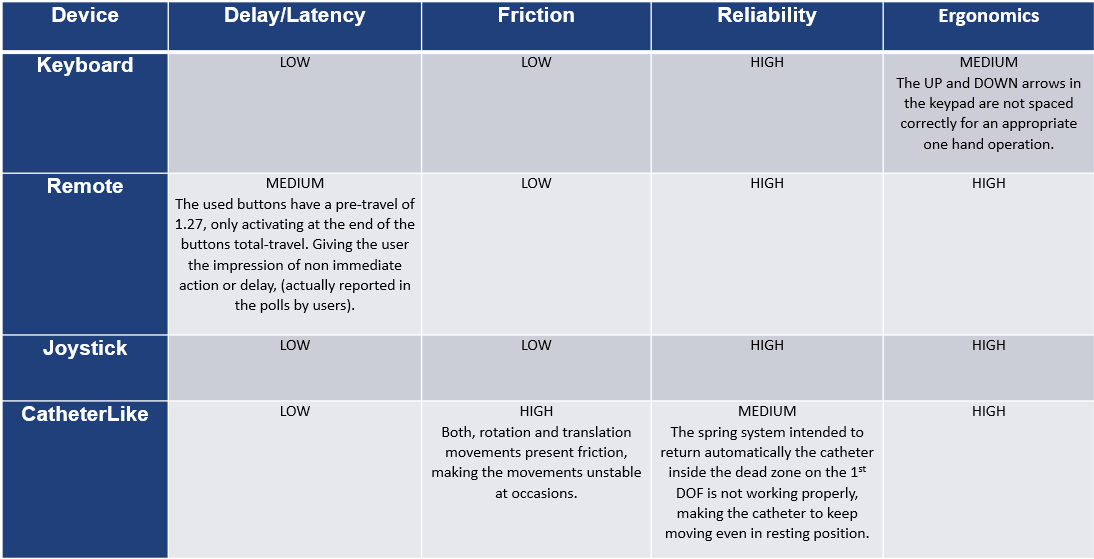
\includegraphics[width=1.0\textwidth]{img/devcomp.PNG}
   \caption{Devices qualitative table from users experience}
   \label{img:devcomp}
\end{figure}

\begin{figure}[ht]
   \centering
   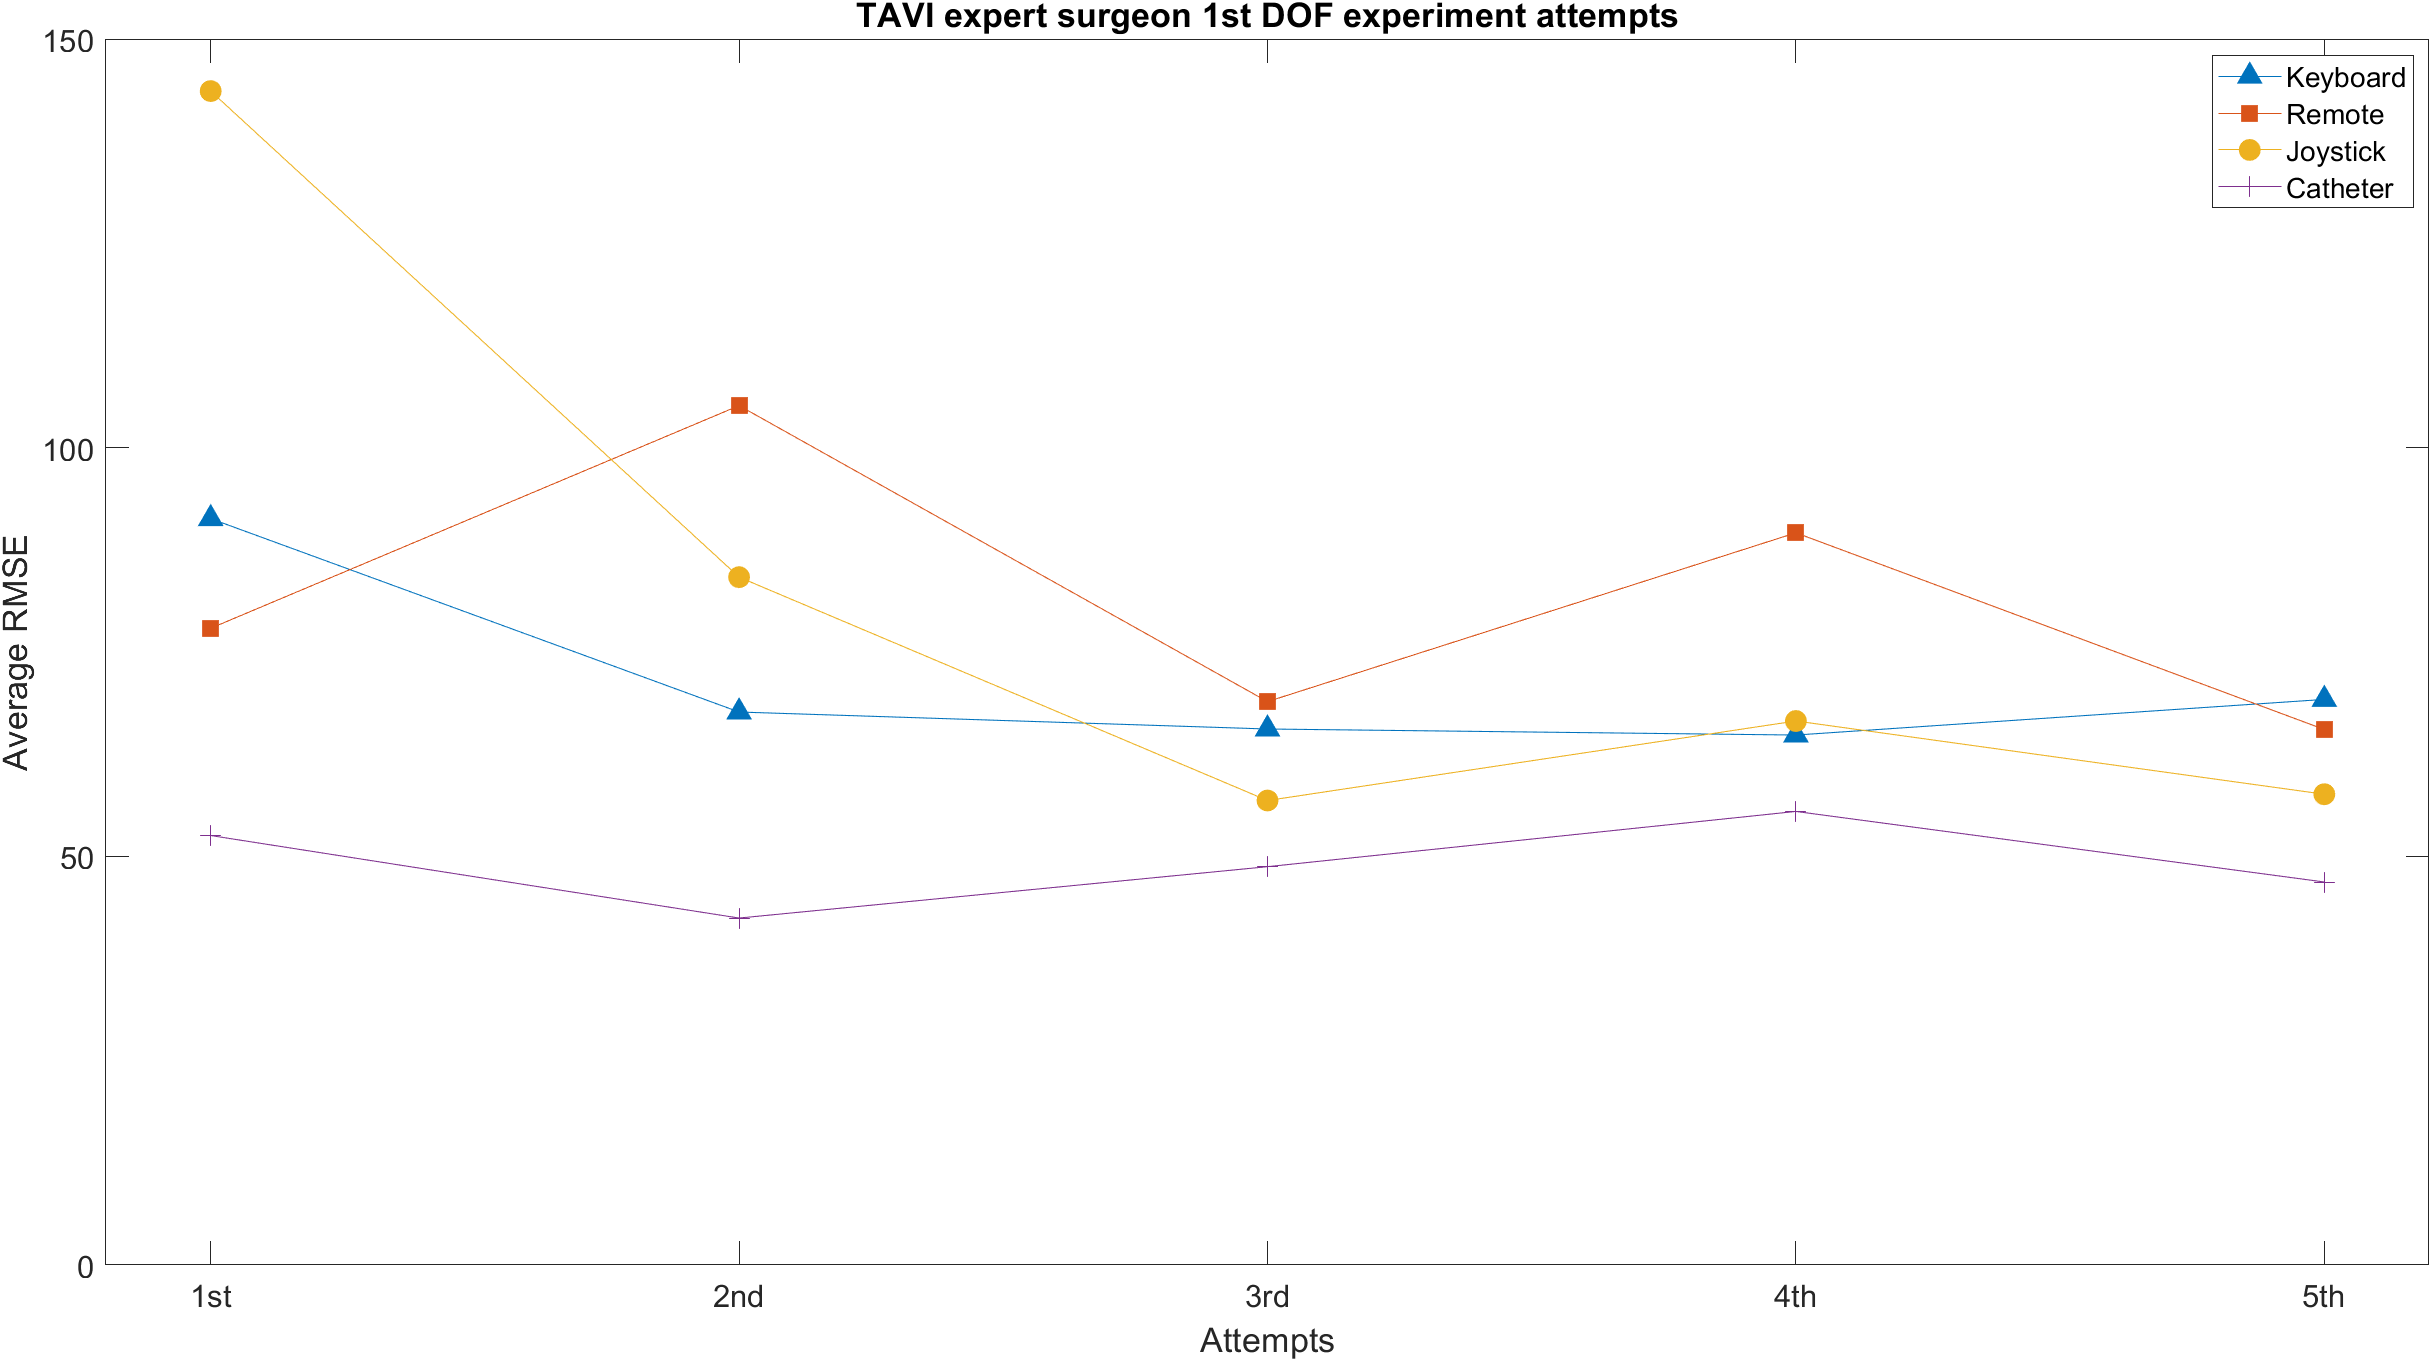
\includegraphics[width=1.0\textwidth]{img/surgat.PNG}
   \caption{Attempts of the expert TAVI surgeon in the 1st DOF experiment}
   \label{img:surgeat}
\end{figure}
\clearpage

\section{Future work} \label{futurework}
Explore different functions for how the velocity over time is incremented in the PressedTime-Velocity mapping, for this thesis work a linear function was used.\\

Explore different mapping functions for the analogical sensor devices in the Position-velocity mapping, for this thesis work a linear function was used.\\

Explore feedback strategies for the possibility of making the devices haptic.\\

Explore the possibility to have two master devices, adding a detachable secondary master device.\\

